\documentclass[tikz]{standalone}
\usepackage{tikz}
\usepackage{pgfplots}

\begin{document}

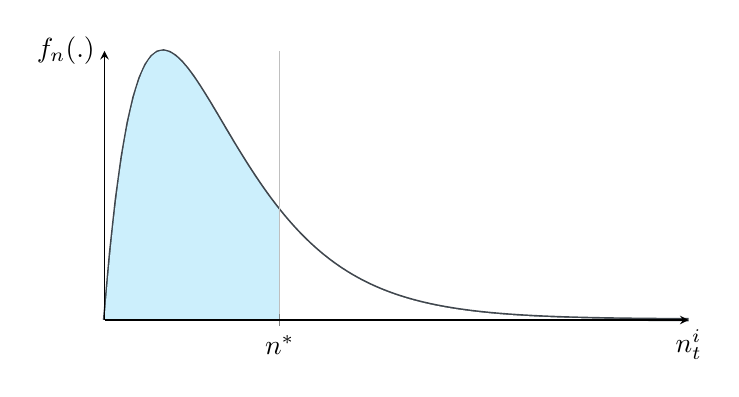
\begin{tikzpicture}[
    declare function={gamma(\z)=
    2.506628274631*sqrt(1/\z)+ 0.20888568*(1/\z)^(1.5)+ 0.00870357*(1/\z)^(2.5)- (174.2106599*(1/\z)^(3.5))/25920- (715.6423511*(1/\z)^(4.5))/1244160)*exp((-ln(1/\z)-1)*\z;},
    declare function={gammapdf(\x,\k,\theta) = 1/(\theta^\k)*1/(gamma(\k))*\x^(\k-1)*exp(-\x/\theta);}
]

\begin{axis}[
  no markers, domain=0:9, samples=100,
  axis lines=left, xlabel=$n_t^i$, ylabel=$f_n(.)$,
  every axis y label/.style={at=(current axis.above origin),anchor=east},
  every axis x label/.style={at=(current axis.right of origin),anchor=north},
  height=5cm, width=9cm,
  xtick={6.0}, ytick=\empty,
  xticklabels={$n^*$},
  %xticklabels={$\bar n (\theta_t)$},
  enlargelimits=false, clip=false, axis on top,
  grid = major
  ]

\addplot [very thick,cyan!20!black,domain=0:20] {gammapdf(x,2,2)};
\addplot [fill=cyan!20, draw=none, domain=0:6.0] {gammapdf(x,2,2)} \closedcycle;
\addplot [very thick, fill=white!20!white, draw=none, domain=6.01:20] {gammapdf(x,2,2)} \closedcycle;


\end{axis}
\end{tikzpicture}
\end{document}